\chapter{Relating Different Instruction Sets}
\label{ch:cross-isa}

An A0 state cannot equal an RV64 state or an x86-64 state. Their register
files have different names and sizes. Their program counters visit different
addresses. Their instructions occupy different byte sequences. A0 and
x86-64 expose condition state that base RV64I does not possess. Literal state
equality would reject every useful comparison before execution began.

Cross-ISA reasoning replaces equality with a relation. The relation says which
machine objects represent the same input, where corresponding results must
appear, which memory regions match, how control locations line up, and which
state may differ. A simulation then shows that execution preserves this shared
meaning even when the machines take different numbers and shapes of steps.

\begin{keyidea}[title={Relate meaning, not register names}]
A cross-machine theorem needs an input relation, control-point relation,
memory relation, outcome relation, and output relation. It may deliberately
ignore scratch registers or condition state, but only after showing that the
rest of the allowed computation cannot expose those differences.
\end{keyidea}

\section{Why translation needs more than matching answers}

Programs have crossed machine boundaries since assemblers, compilers, and
emulators first separated a programmer's operation from one machine's code.
Retargeting a compiler asks whether different instructions implement the same
source operation. Emulation asks whether one machine can reproduce another's
steps. Binary translation asks whether already encoded code can move between
architectures. Hardware verification often compares an implementation with a
simpler reference machine.

Today the same question appears in verified compilers, portable cryptography,
instruction lifting, migration tools, and superoptimization. A translator can
produce the expected result on test inputs while mishandling a fault, high
address, condition bit, calling convention, or loop exit. A destination-only
comparison is a useful test; it is not a cross-machine correctness theorem.

The abstraction level also matters. A source-language integer may correspond
to a word in each machine. A source function may correspond to entire machine
routines. One abstract step may require several target instructions, while one
target instruction may combine several abstract operations. The proof should
choose a level at which the relation is both true and useful.

\begin{archive}[title={A relation is a small bilingual dictionary}]
The relation does not translate every fact in either machine. It records the
facts needed for one shared computation: this register carries the input,
these bytes represent the same array, these locations are corresponding loop
heads, and these outcomes mean the same kind of completion.
\end{archive}

\subsection{Three translation questions that should not be collapsed}

Compiler correctness, instruction lifting, and binary translation all cross
semantic boundaries, but they begin with different objects. A compiler starts
from a source-language program and usually relates whole behaviors through
several intermediate languages. A lifter translates decoded machine
instructions into an intermediate form for analysis. A binary translator
turns one encoded machine program into another executable program.

In compiler verification, the source may leave implementation choices unspecified or
declare some executions outside its guarantees. The target has concrete words,
registers, and faults. A semantic-preservation theorem must state how source
behaviors correspond to target behaviors; CompCert is a major demonstration of
this style at realistic scale \autocite{leroy2009compcert}.

A lifter has a more local initial question: does executing the lifted
intermediate statement reproduce the decoded instruction's architectural
effect under a state relation? If the lifter drops flags, faults, or address
width, its intermediate language may be too weak for later analyses. A useful
lifting theorem therefore names both the translated effect and the observation
under which omitted state is safe.

A binary translator owns control layout as well as local operations. Expanding
one source instruction into several target instructions moves branch targets
and may require scratch storage. Calls and returns must respect a target ABI.
Code addresses embedded in data or calculated at run time can make relocation
observable. Local instruction lemmas are necessary, but a whole-program
control relation is what composes them.

\begin{table}[htbp]
\centering
\caption{Related translation tasks begin and end at different semantic levels.}
\begin{tabular}{@{}p{0.21\textwidth}p{0.31\textwidth}p{0.36\textwidth}@{}}
\toprule
Task & Source and target & Central proof question \\
\midrule
Compiler & source language to machine code & are allowed source behaviors preserved? \\
Lifter & decoded instruction to intermediate statement & does one lifted movement match one machine movement? \\
Binary translator & encoded machine program to encoded machine program & do local matches compose through control and procedure context? \\
Emulator & guest states to host execution & does each guest movement have a faithful finite host realization? \\
\bottomrule
\end{tabular}
\end{table}

The A0-to-real-ISA direction in this book resembles a small reference-machine
refinement. It does not claim that A0 is a source language or that either real
machine implements every A0 behavior. The candidate slices and relations are
chosen per theorem. Keeping that scope narrow is what makes the proof
inspectable.

\subsection{RISC and CISC are shapes, not proof shortcuts}

RV64I often exposes operations through regular fixed-width instructions and
explicit registers. Selected x86-64 instructions may combine a memory access
with arithmetic, use a destination as an implicit source, or update a rich
status register. These broad RISC and CISC tendencies change useful cut points.
They do not determine which proof is easier.

Consider adding a memory word to an \keyterm{accumulator}, a register that
holds the running result. An RV64 implementation may
use a load followed by register addition. One selected x86 form may add a
memory operand directly. The relation can compare the RV64 intermediate loaded
word with the internal value consumed by the x86 instruction, or it can place
cut points before and after the whole movement. The latter avoids inventing an
architectural x86 state that does not exist between load and add.

Conversely, a single architectural instruction can have many cases. An x86
memory operand may require variable-length decode, address calculation,
segment and mode assumptions, range checks, a memory read, arithmetic, status
updates, and instruction-length advancement. Two RV64 instructions may give
the proof more visible intermediate states even though the program has more
steps. Step count and semantic complexity are different measures.

\begin{example}[title={Choose a relation boundary that both machines possess}]
Relate the states immediately before an RV64 load-plus-add pair and an x86
memory-source add. Execute each complete segment. At the endpoints, require
equal accumulator words, corresponding next control points, preserved related
memory, and normal outcomes. Do not require a fictional x86 state halfway
through its atomic architectural instruction.
\end{example}

The same principle applies in reverse when one architecture exposes an effect
through a register and another through flags. Relate the Boolean or arithmetic
meaning at a point where both are available. Architecture-family labels help
predict where mismatches may appear; only decoded semantics and a stated
relation settle the theorem.

This view also explains why the book studies both families from one scalar
foundation. A0 supplies a compact semantic vocabulary, not a claim that every
real instruction decomposes into one canonical RISC-like sequence. Sometimes
one A0 movement matches several real instructions. Sometimes one real
instruction matches several A0 movements at once. The relation may choose
either grouping when the endpoints, intermediate fault policy, and progress
argument are explicit. Universality comes from the relational method, not from
making one architecture imitate the surface form of another.

That flexibility is disciplined rather than arbitrary: every chosen grouping
must still preserve the declared observation, expose its freedom clauses, and
survive a control aimed at the semantic difference it intentionally crosses.

\section{Anatomy of a cross-machine state relation}

Let \(S_A\), \(S_R\), and \(S_X\) range over A0, RV64, and x86-64 states. A
relation for one routine can be written as a conjunction of smaller clauses.

\begin{enumerate}
\item \emph{Value relation}: selected registers or memory objects carry equal
width-\(w\) words or related mathematical readings.
\item \emph{Memory relation}: corresponding byte intervals contain equal or
translated bytes, with declared base addresses and ownership.
\item \emph{Control relation}: each machine's program counter belongs to a
named corresponding control point.
\item \emph{Condition relation}: required predicates agree, even if one
machine stores them in flags and another recomputes them.
\item \emph{Outcome relation}: running, normal return, and selected traps
correspond under the theorem's policy.
\item \emph{Frame relation}: stack pointers, saved locations where execution
continues, arguments,
results, and preserved state satisfy the chosen ABI slice when procedures are
in scope.
\item \emph{Freedom clause}: scratch registers, dead flags, code addresses,
and private bytes not mentioned above may differ.
\end{enumerate}

\begin{figure}[htbp]
\centering
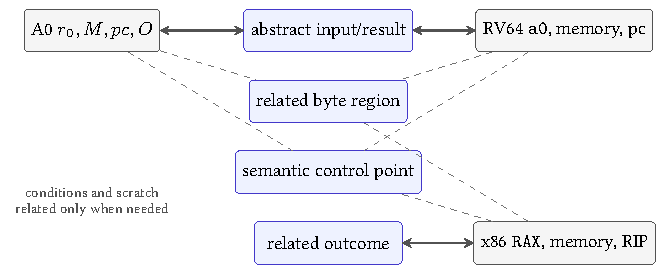
\includegraphics[width=0.94\textwidth]{figures/cross-state-relation}
\caption{A relation aligns selected meanings across three unlike states. Gray
components may differ only when the theorem and its contexts leave them free.}
\figalt{A0 r0, RV64 a0, and x86 RDI or RAX map to one abstract value; memory, control, and outcomes also map while scratch differs.}
\label{fig:cross-state-relation}
\end{figure}

The freedom clause is as important as the required clauses. Without it, readers may
assume either that every omitted component must match or that every omission
is harmless. A typed relation should list ignored and scratch state explicitly
and prevent the final observation from reading it.

\begin{definition}[title={Control points name related moments}]
A control point is a semantic location such as routine entry, branch decision,
loop head, memory update, or normal exit. It maps to one or more concrete
program-counter values in each implementation. States at matching control
points may be related even when states between them have no direct partner.
\end{definition}

Numeric program-counter equality is usually irrelevant across ISAs. What
matters is that A0 at its \emph{decision} label corresponds to RV64 at its
branch and x86-64 after the flags used by its conditional jump have been
established. The relation can pair those distinct addresses through one
control-point tag.

\subsection{Design the observation before the relation}

A relation can become needlessly strong when its author starts by pairing
registers. Begin instead with the client-visible contract. Does the caller
observe one result word, a returned memory region, normal versus trapped
termination, preserved registers, or the next continuation? The relation then
needs enough state to carry those observations through the computation.

Suppose a routine receives two words and returns their sum. A result-only test
might compare A0 \(r_0\), RV64 \code{a0}, and x86 \code{rax} at exit. A
procedure theorem also relates entry arguments, stack discipline,
continuations, and preserved registers. A contextual-replacement theorem may
need condition state if a surrounding private convention reads it. These are
three different claims about the same instruction sequences.

\begin{table}[htbp]
\centering
\caption{Observation strength determines relation strength.}
\begin{tabular}{@{}p{0.24\textwidth}p{0.31\textwidth}p{0.34\textwidth}@{}}
\toprule
Claim & Required relation & May remain free \\
\midrule
Result computation & inputs, result, normal outcome & scratch and continuation \\
Callable routine & arguments, result, frame, continuation & caller-saved scratch \\
Contextual replacement & every state later read by allowed contexts & state unreachable to those contexts \\
\bottomrule
\end{tabular}
\end{table}

After choosing the observation, write a control-point table. Each row names a
logical moment. Each machine column gives the concrete address or decoded
instruction associated with that moment. The last column states the relation
that must hold there. Gaps in this table often reveal that one machine performs
an operation earlier or later than the others.

\begin{figure}[htbp]
\centering
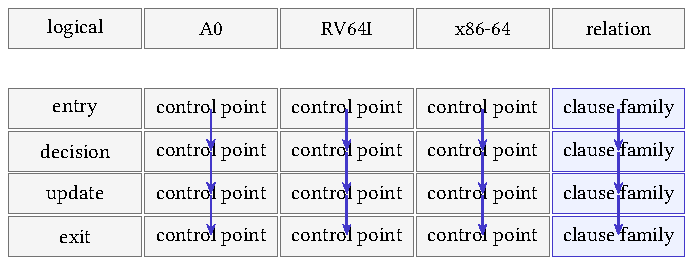
\includegraphics[width=0.9\textwidth]{figures/control-point-table-flow}
\caption{A control-point table turns three address spaces into one sequence of
logical moments. Local proofs connect adjacent rows.}
\figalt{Rows labeled entry, decision, update, and exit cross three machine columns, with arrows between rows and one relation column.}
\label{fig:control-point-table-flow}
\end{figure}

The table is not itself a proof. It is a proof plan. For every adjacent pair,
ask which instructions execute, which relation clauses they read, which clauses
they restore, and which intermediate states remain intentionally unrelated.
This turns a broad cross-ISA claim into finite local obligations.

\begin{tryit}[title={Make freedom executable}]
Choose one scratch register omitted at exit. Change its initial value while
holding every related component fixed. Then append a context that reads it.
Either the context must be excluded, or the relation must be strengthened.
\end{tryit}

\section{Memory correspondence needs addresses and ownership}

Equal bytes at numerically equal addresses are only one possible memory
relation. A translated routine may place the source array at base \(a\) and
the target array at base \(b\). For a length \(n\), a simple relation is
\[
  M_A[a+i]=M_T[b+i]
  \quad\hbox{for every }0\leq i<n.
\]
Outside those intervals, the theorem may require equality, preservation, or
nothing, depending on ownership and observation.

Loads also need address correspondence. If A0's effective address is
\(R_A[r_1]+d_A\) and RV64's is \(R_R[x_5]+d_R\), the input relation must imply
that both select corresponding offsets within the related regions. Equal loaded
words then follow from byte agreement, width, and matching little-endian join
rules.

\begin{proofkit}[title={Related bytes give related little-endian words}]
Assume width \(w=8k\), corresponding bases \(a,b\), and
\(M_A[a+i]=M_T[b+i]\) for \(0\leq i<k\). Each load joins byte \(i\) with
weight \(2^{8i}\). Term-by-term equality gives equal sums modulo \(2^w\), so
the loaded words are equal. The proof fails if widths, byte order, or accessed
offsets differ.
\end{proofkit}

Stores require a frame condition. Corresponding stores should write related
bytes inside their owned intervals, and every caller-owned observed byte
outside those intervals should remain unchanged. Merely comparing the written
result misses collateral memory damage.

\begin{warning}[title={A memory relation must survive aliasing}]
Two symbolic base registers may identify overlapping ranges. If a proof treats
them as disjoint, nonaliasing belongs in the input relation. If overlap is
allowed, the simulation must account for the shared bytes and write order.
\end{warning}

\section{Forward simulation permits unequal step counts}

A \keyterm{forward simulation} begins with related states. Whenever the source
makes a matched step or segment, the target makes zero or more steps to a state
related to the source successor. Repeating this argument follows the source
execution forward.

Allowing zero target steps is \keyterm{stuttering}. It handles an abstract
state change that the target already represents, bookkeeping steps ignored by
the relation, or different placement of control points. To rule out a target
that stutters forever while the source progresses, a simulation may require a
well-founded rank that decreases on zero-progress matches.

\begin{figure}[htbp]
\centering
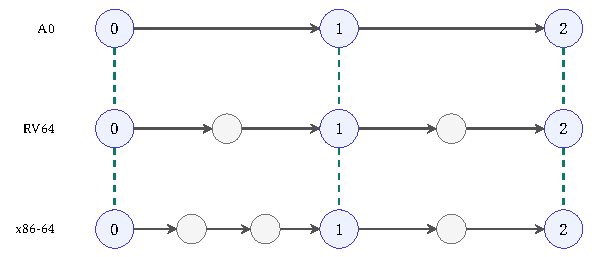
\includegraphics[width=0.9\textwidth]{figures/stuttering-simulation}
\caption{Forward simulation relates synchronization points, not every row.
One A0 segment can match several RV64 or x86-64 instructions.}
\figalt{A0 has three related states; RV64 and x86 paths have extra intermediate states, with vertical relation lines only at control points.}
\label{fig:stuttering-simulation}
\end{figure}

For finite straight-line routines, the proof can divide code into segments
between control points. For loops, the relation must be invariant at every
revisit, and progress or termination needs a separate argument. For branches,
predicate agreement ensures that related states select corresponding edges.

\begin{proofkit}[title={From local simulation to an endpoint relation}]
Assume entry states are related. For each source segment between control points,
the target has a finite matching segment whose endpoint restores the relation.
Induct over the source segments. The base case is entry. The local simulation
supplies the next related pair in the inductive step. At a terminal source
point, the outcome clause and output relation therefore hold for the target
endpoint. Looping executions additionally require a coinductive or invariant
argument rather than finite induction over a fixed segment count.
\end{proofkit}

Forward simulation is directional. It shows that target behavior can be
matched by the specification under the selected orientation only if the step
clause is stated that way. With nondeterminism, reverse simulation may be
needed to exclude extra target behaviors. Our selected scalar examples are
deterministic, but the direction should still appear in the theorem.

\subsection{Safety, progress, and termination are separate transfers}

A local simulation usually establishes a safety shape: if related execution
reaches the next cut point, the new states are related. That conditional does
not yet say that the target reaches the point. A target might trap, diverge in
an internal loop, or stop because a runner exhausted its bound. Progress adds
the fact that a legal matched segment can take a next movement. Termination
adds a global argument that repeated movements reach an exit.

For a deterministic finite straight-line segment, progress often follows by
executing each decoded instruction and showing that no premise for a trap is
violated. For a loop, a rank or source termination theorem is also needed. If
one source iteration matches a finite target segment of at least one step, source
termination can transfer. If zero-step matches are allowed, the proof must
show that they cannot postpone progress forever.

Outcome refinement needs the same separation. One policy may require normal
return to match normal return and every selected trap to match its counterpart.
Another may prove only that normal source executions have normal target
matches. The second theorem is weaker and can still be useful, but it cannot be
quoted as universal behavioral equivalence.

\begin{definition}[title={Segment simulation obligation}]
For related source and target states at control point \(q\), a segment
obligation names a source path, a finite target path, their required entry
premises, the next control point \(q'\), and the relation restored at their
endpoints. It also names every failure outcome permitted before \(q'\).
\end{definition}

The word ``finite'' needs evidence. In a hand proof, the target path may be a
fixed list of instructions. In a symbolic proof, a rank or bounded internal
semantics may establish that the path is finite. A trace bound chosen by the checker is only
a search resource until the theorem connects it to program structure.

\subsection{When a reverse direction is required}

Imagine a target program that returns the correct result for every related
source run but also has an extra path that leaks into an unrelated successful
result. A source-to-target existence statement can ignore the extra path.
Behavioral equivalence cannot. A reverse simulation, determinism argument, or
set-inclusion proof must rule it out.

Our three scalar machines are deterministic once bytes, state, and fault rules
are fixed. This makes a forward simulation stronger: the target does not get to
choose another successor. The theorem should still cite determinism rather
than inherit it from intuition. Later models with concurrency, interrupts, or
underspecified behavior lose that shortcut.

\section{A three-machine absolute-value routine}

Let \(x\) be a width-\(w\) word and \(\langle x\rangle_s\) its signed reading.
The mathematical absolute value lies outside the signed width-\(w\) range when
\(x\) is the minimum signed value \(-2^{w-1}\). We therefore choose one of two
honest specifications:

\begin{enumerate}
\item modular absolute value, which returns \(x\) when nonnegative and
\(-x\bmod 2^w\) otherwise; or
\item mathematical absolute value under precondition
\(\langle x\rangle_s\ne-2^{w-1}\).
\end{enumerate}

The worked proof uses the second. The precondition is not a decoder fact or an
ABI rule. It is the domain on which a positive signed result represents the
mathematical absolute value.

Use these schematic implementations:

\begin{codelisting}[language={},caption={A0 absolute value, with r1 initialized to zero}]
cmp       r0, r1
branch.ge done
sub       r0, r1, r0
done:
\end{codelisting}

\begin{codelisting}[language={},caption={RV64I absolute value}]
bge  a0, x0, done
sub  a0, x0, a0
done:
\end{codelisting}

\begin{codelisting}[language={},caption={x86-64 absolute value in the selected local contract}]
mov  rax, rdi
test rax, rax
jns  done
neg  rax
done:
\end{codelisting}

The x86 listing is schematic Intel syntax for selected 64-bit forms. The
chapter compares decoded semantics, not exact bytes. Machine-code evidence
would additionally require source-pinned encodings and instruction lengths
\autocite{riscv2026unpriv,intel2026sdm2}.

At entry, relate A0 \(r_0\), RV64 \code{a0}, and x86-64 \code{RDI} to the
same input word \(x\). Require A0 \(r_1=0\). The x86 destination \code{RAX}
is initially free because its first instruction copies the input. Relate
running outcomes, valid code, and routine-entry control points. Memory is
unchanged by all three routines and may be required equal or separately
preserved under the local contract.

At the decision point, A0's comparison establishes \(N=V\) exactly for
signed \(x\geq0\) in this comparison. x86 \code{test} establishes the sign
predicate read by \code{jns}. RV64 \code{bge} compares \code{a0} directly
with \code{x0}. Thus all three choose their done edge exactly when the common
signed reading is nonnegative.

\begin{figure}[htbp]
\centering
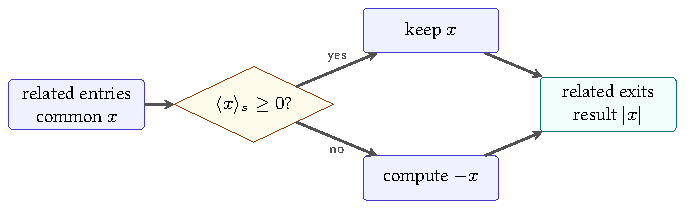
\includegraphics[width=0.88\textwidth]{figures/abs-control-points}
\caption{The absolute-value simulation splits on one shared signed predicate.
Each path restores a common result relation at \emph{done}.}
\figalt{Related entries lead to a shared x nonnegative decision; the positive path keeps x, the negative path computes minus x, and both reach related exits.}
\label{fig:abs-control-points}
\end{figure}

\begin{proofkit}[title={Reader simulation for absolute value}]
Take arbitrary related entries satisfying the minimum-value exclusion. Split
on the common signed reading. If \(x\geq0\), predicate agreement sends all
three routines directly to \emph{done}; their result locations contain \(x\),
which equals \(|x|\). If \(x<0\), all take the negation path. A0 and RV64
subtract \(x\) from zero; x86-64 negates its copied word. Fixed-width arithmetic
gives the same word \(-x\bmod2^w\). The precondition makes its signed reading
positive and equal to \(|x|\). At \emph{done}, the result words, outcomes, and
preserved memory are related. Scratch condition state may differ.
\end{proofkit}

For the excluded minimum word, each modular negation returns the same bit
pattern as the input. The modular-refinement claim still holds. The
mathematical-positive-result claim fails because \(2^{w-1}\) has no positive
signed width-\(w\) representation. This counterexample shows why the input
domain belongs beside the relation.

\subsection{Expand the branch proof into local movements}

The reader proof above compresses setup, decision, and update. Expanding those
movements shows exactly where architecture-specific facts enter.

At A0 entry, \(r_1=0\) is a premise supplied by the harness. The comparison
writes condition state without changing \(r_0\). Its signed predicate follows
from the A0 subtraction rule. At RV64 entry, \code{x0} supplies zero and the
branch compares register readings directly; there is no setup condition state.
At x86 entry, \code{mov rax,rdi} copies the input, then \code{test rax,rax}
sets the sign and zero information read by \code{jns}.

The decision relation can therefore be written as
\[
 D(x,S_A,S_R,S_X)
 \quad\hbox{iff}\quad
 \begin{array}{l}
 R_A[r_0]=R_R[a0]=R_X[rax]=x,\\
 (N_A=V_A)\quad\Longleftrightarrow\quad \langle x\rangle_s\ge0,\\
 \mathit{SF}_X=0\quad\Longleftrightarrow\quad \langle x\rangle_s\ge0,
 \end{array}
\]
with the RV64 branch evaluating the last mathematical predicate from its two
source registers. The formula does not equate A0 \(N\) with x86 \(SF\): A0's
signed comparison uses \(N=V\), while x86 \code{test} clears overflow and
records the input high bit in \(SF\). It equates the question they answer.

On the negative path, the update lemma assumes \(\langle x\rangle_s<0\). A0
and RV64 compute \(0-x\) by subtraction. x86 \code{neg} computes the same
modular word. The minimum-value exclusion is not needed for word equality; it
is needed only when converting that word to the positive mathematical value
\(-\langle x\rangle_s\). Keeping those proof steps separate shows that the
modular theorem is strictly broader.

\begin{table}[htbp]
\centering
\caption{Local obligations in the absolute-value simulation.}
\begin{tabular}{@{}p{0.2\textwidth}p{0.7\textwidth}@{}}
\toprule
Movement & Main fact \\
\midrule
Entry setup & all three result paths begin from the common word \(x\) \\
Predicate & each machine selects the nonnegative edge exactly for \(\langle x\rangle_s\ge0\) \\
Keep path & result locations retain \(x\) and frames remain intact \\
Negate path & all result locations receive \(-x\bmod2^w\) \\
Exit & outcome, result observation, continuation policy, and memory agree \\
\bottomrule
\end{tabular}
\end{table}

Each row admits a focused negative control. Remove the x86 move to break entry
setup. Change one signed predicate to unsigned to break the decision. Add an
unexpected write to break a frame. Negate the wrong register to break update.
Redirect the return to break exit. These controls diagnose more precisely than
one end-to-end expected result.

\begin{tryit}[title={Trace both paths at width four}]
Use inputs \code{0011}, \code{1101}, and \code{1000}. Record the shared signed
predicate, each path, and final word. Identify which input satisfies modular
absolute value but violates the mathematical-range specification.
\end{tryit}

\section{Condition state can be related and then forgotten}

A0 and x86-64 need condition information at their branches. RV64I does not
retain an arithmetic-flags register. The simulation relation should therefore
be control-point specific. At the decision point, relate the Boolean question
``is the common signed input nonnegative?'' to A0's \(N=V\), RV64's register
comparison, and x86-64's selected sign condition. At the routine exit, omit
conditions when the output contract does not expose them.

Forgetting flags at exit is sound only for contexts that establish their own
required condition state before reading it. If the x86 caller branches on
flags immediately after the routine under a private convention, those flags
belong in the output relation. Ordinary ABI rules and a custom local contract
can expose different state.

\begin{sidebar}[title={Abstraction can change across control points}]
The entry relation may ignore destination scratch. The decision relation may
require predicate agreement. The exit relation may forget conditions but
require a result and continuation. One monolithic equality is less useful than
a family of relations indexed by semantic control point.
\end{sidebar}

Undefined or form-specific flags require special care. A relation must not
read an architectural value the selected instruction leaves undefined. It may
instead relate only the predicate whose source rules define it, choose another
instruction form, or restrict the context so that the undefined component is
unobserved.

\section{Faults and outcomes must correspond}

The absolute-value routine uses registers only, but instruction fetch, illegal
encoding, invalid targets, and terminal input states can still affect execution
in a complete model. A cross-ISA theorem normally restricts entry to valid
code and running outcomes, then proves corresponding normal exits.

Memory routines need stronger fault agreement. One ISA may permit an unaligned
access that another traps or decomposes. A theorem can require aligned valid
ranges, relate both trap classes, or refine a source operation into a checked
target sequence. Silently discarding inputs on which only one side traps
changes the precondition and must be visible.

\begin{warning}[title={Shared normal results do not repair unequal faults}]
If one implementation traps before producing its result and another returns,
their normal-result formulas may still be identical. The behavior
relation fails unless the theorem explicitly uses a weaker policy that is
appropriate for its context.
\end{warning}

Likewise, related termination is not established by checking a fixed trace
bound. A simulation can transfer termination from a source to a target when
each source progress segment has a finite target match and stuttering cannot
continue forever. If the target may take an unbounded internal loop between
control points, endpoint tests do not exclude divergence.

\section{Building the Axeyum cross-ISA route}

The current Axeyum checkout does not yet contain reusable A0, RV64I, or
x86-64 decoder-and-step packages or typed cross-machine relations. This
chapter therefore specifies the required route without presenting the
absolute-value simulation as machine-established evidence.

Implementation should proceed in dependency order:

\begin{enumerate}
\item complete and test A0 state, decoder, step, and bounded-run packages;
\item implement a source-pinned RV64I slice for the exact branch, subtraction,
and jump forms used by the selected routine;
\item implement a source-pinned x86-64 slice for the exact move, test,
conditional jump, negation, and return forms used;
\item define typed control-point relations with register, memory, condition,
program-counter, outcome, and freedom clauses;
\item check each local simulation segment and compose the endpoint theorem;
\item decode and replay every satisfiable counterexample through all affected
executable semantics.
\end{enumerate}

The relation should be data, not an informal callback hidden in a test. A
manifest names semantic-package digests, source revisions, program bytes or
decoded programs, control-point map, precondition, relation schema, observation,
and expected evidence class. The checker reports which clause first failed.

\begin{example}[title={Negative controls for the absolute-value simulation}]
Swap signed \code{bge} for unsigned \code{bgeu}; invert one branch; negate the
wrong register; omit the x86 copy; relate \code{RDI} rather than \code{RAX} at
exit; admit the minimum signed word while claiming a positive mathematical
result; or let one implementation write an observed memory byte. Each mutation
has a small witness and should fail a distinct relation or semantic clause.
\end{example}

At small widths, exhaustive enumeration can check every related entry and
both paths. At width 64, a solver can search for a violation of each segment
or the composed endpoint relation. A model must become three concrete traces
and a failed relation clause. An unsatisfiable formula needs its exact digest
and the strongest available certificate or kernel route; a solver message
alone does not create a cross-ISA theorem.

Counterexample triage should move from the outside inward. First validate that
the model satisfies the serialized precondition. Then construct concrete
machine states and check the entry relation. Decode the bound program bytes.
Replay each segment. Finally compare the reported failed clause with the
concrete endpoint values. A failure at an earlier stage invalidates the later
interpretation.

\begin{figure}[htbp]
\centering
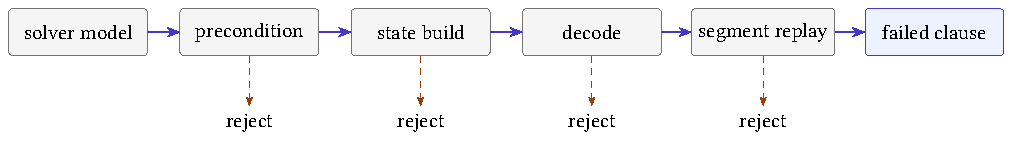
\includegraphics[width=0.9\textwidth]{figures/cross-isa-counterexample-triage}
\caption{A solver assignment becomes a cross-ISA counterexample only after it
survives construction, decoding, replay, and relation checking.}
\figalt{A funnel passes a solver model through precondition, state construction, decode, segment replay, and failed relation clause; side arrows mark rejection.}
\label{fig:cross-isa-counterexample-triage}
\end{figure}

This order distinguishes a genuine semantic disagreement from a generator bug.
For example, a symbolic model may assign an out-of-range register index that a
real decoder rejects. It may describe code bytes different from those in the
manifest. It may satisfy a formula whose branch target uses the wrong base.
None is evidence that the two actual machine programs disagree; each is
evidence that a binding layer needs repair.

\begin{goingdeeper}[title={Why two matching formulas are not enough}]
Encoding \(y=x\) for nonnegative inputs and \(y=-x\) otherwise on both sides
checks a shared mathematical formula. It does not establish decoding,
instruction effects, branch targets, scratch writes, memory preservation,
traps, or control-point progress. The formula becomes useful evidence only
after executable source-pinned semantics connect machine bytes to it.
\end{goingdeeper}

The introductory Python or PyO3 API can expose named routines, widths,
relations, observations, and returned counterexample traces. Rust should own
the typed semantic objects, digests, solver encoding, and replay. Convenience
at the boundary should reduce setup work, not erase which route and scope
supported the result.

\subsection{A beginner route should expose the relation}

An introductory interface should not begin with a Boolean function named
\code{equivalent}. It should let the reader construct the three entry states,
inspect the control-point map, execute one segment, and ask which relation
clauses hold. Only then should it offer a composed comparison.

\begin{codelisting}[language=Python,caption={Illustrative future relation-first interface}]
case = abs_case(width=8, value=0xfd)
states = case.entry_states()

print(case.relation("entry").explain(states))
segments = case.step_to("decision", states)
print(case.relation("decision").explain(segments.ends))

report = case.compare_to_exit()
print(report.first_failed_clause())
\end{codelisting}

The sketch is not a current Axeyum import. Its design requirement is important:
\code{explain} reports satisfied and failed clauses with concrete values. A
negative control that changes RV64 \code{bge} to \code{bgeu} should point to
predicate or control disagreement, not return an undifferentiated false value.

At the Rust layer, a control point can be an enumeration and each relation a
typed structure containing value, memory, control, condition, outcome, frame,
and freedom clauses. Segment checkers consume decoded traces and return their
endpoint states. Solver formulas are derived from the same structures, and any
model is replayed by those executable segment checkers.

Chapter 15 provides the next scale test. Its XOR loop reuses this machinery but
adds memory, a loop invariant, and repeated cut points. Building the small
absolute-value route first would therefore create reusable semantics rather
than a disposable demonstration.

The relation-first interface also changes how a failed comparison is taught.
Suppose the terminal values disagree. A flat comparator can report only the
two numbers. A structured route asks where the relation last held, which
segment broke it, and which clause failed first. If value correspondence fails
after the decision point while control correspondence still holds, inspect
the selected arithmetic step. If control fails while values remain related,
inspect the predicate and target. If the frame clause fails, look for an
unexpected scratch or memory write even when the selected result is correct.

That diagnosis is more than a convenience. It mirrors the composition proof.
Each segment has premises, a local movement, and an endpoint relation. The
first broken endpoint identifies the first local lemma that cannot be reused.
A minimized counterexample can then retain only the state components named by
that lemma, making the difference small enough to replay by hand.

\begin{sidebar}[title={A counterexample should name its control point}]
For cross-machine work, an input alone is rarely an adequate counterexample.
Retain the three entry states, the last related control point, the first
failed relation clause, and the decoded steps that crossed the gap. Those
facts turn disagreement into a repairable semantic question.
\end{sidebar}

\section{Where the cross-ISA model stops}

This chapter covers deterministic scalar architectural routines over selected
integer instructions. It excludes floating point, vector state, atomics,
concurrency, weak memory, privilege, interrupts, exceptions across frames,
self-modifying code, dynamic linking, timing, microarchitectural state,
speculation, and side-channel observations.

The worked routine is a semantic teaching instance, not evidence that current
Axeyum can decode or execute its real machine code. It also does not claim that
the three instruction sequences have equal cost. Chapter 13 defines candidate
languages and costs; Chapter 15 develops a richer scalar routine through the
whole evidence chain.

Within this boundary, a state relation lets unlike machines share one exact
story. Their bytes, registers, flags, and step counts remain different. The
simulation shows why those differences still converge on the same declared
meaning.

\section{Exercises}

\begin{enumerate}
\item List the seven clauses of a cross-machine state relation and give one
absolute-value fact belonging to each.

\item Relate A0 \(r_0\), RV64 \code{a0}, and x86-64 \code{RDI} at routine
entry. State the width and signed-reading convention.

\item Explain why x86-64 \code{RAX} may be unconstrained at entry but must be
related at exit in the worked routine.

\item \textbf{Execute.} Trace all three absolute-value routines at width four
for \code{0011}, \code{1101}, and \code{1000}. Include predicate and result
relations at every control point.

\item \textbf{Prove.} Prove the nonnegative branch of the reader simulation,
including program-counter, result, memory, and outcome clauses.

\item Prove the negative branch under the minimum-value exclusion. Identify
the exact step that uses the precondition.

\item \textbf{Break.} Replace RV64 \code{bge} with \code{bgeu}. Find the
smallest-width witness and replay the path difference.

\item State a modular absolute-value specification that includes the minimum
signed word. Explain why its final bit-vector relation holds while a positive
signed-result claim fails.

\item Draw control-point matches for one A0 segment corresponding to two or
more x86-64 steps. Identify the intermediate x86 state intentionally omitted
from the relation.

\item Give a stuttering simulation that would incorrectly permit infinite
target stuttering. Add a natural-valued rank that rules it out.

\item \textbf{Transfer.} Define a memory relation for equal 16-byte arrays at
different base addresses. Include bounds, byte correspondence, ownership, and
outside-memory preservation.

\item Prove that corresponding little-endian bytes produce equal width-32
loads. Then break the proof by reversing one join order.

\item Give an aliasing counterexample to a relation that treats two overlapping
output ranges as independent. State a sufficient nonaliasing premise.

\item Relate A0 and x86 condition state only at the absolute-value decision
point. Explain why the exit relation may omit it under one context and must
retain it under another.

\item Construct one pair of implementations with equal normal results but
different fault behavior. State three possible outcome relations and which
ones accept the pair.

\item \textbf{Prove.} Formalize the local-to-endpoint simulation argument by
induction over a finite list of control-point segments.

\item Design an Axeyum manifest for the three-machine absolute-value routine.
Include source pins, semantic digests, decoded programs, control points,
precondition, relation clauses, observation, and seven negative controls.

\item A returned solver model violates the relation but fails RV64 executable
replay. List possible generator, decoder, and semantic fault classes. Explain
why the model cannot support the claimed counterexample.
\end{enumerate}
